\section{Grid af Kullorsuaq}
I denne underafsnit beskrives fordelingen af arealer i Kullorsuaq. Fordelingen er nødvendigt for at finde ud af hvor meget af cellens ressource skal sendes til et bestemt område i bygden. Ud fra tildeling af ressourcer findes samtidig, hvor mange celler der skal installeres i bygden, så kapacitetsbehovet er overholdt tilfredsstillende.\\

Fordelingen er delt, så antallet af huse/bygninger er rimelig fordelt. Hver tern har en opløsning på 100x100 meter og der er ikke en hus/bygning som står alene i en tern. Fordelingen kan ses på figur \ref{fig:grid}

\begin{figure}[h]
	\centering
	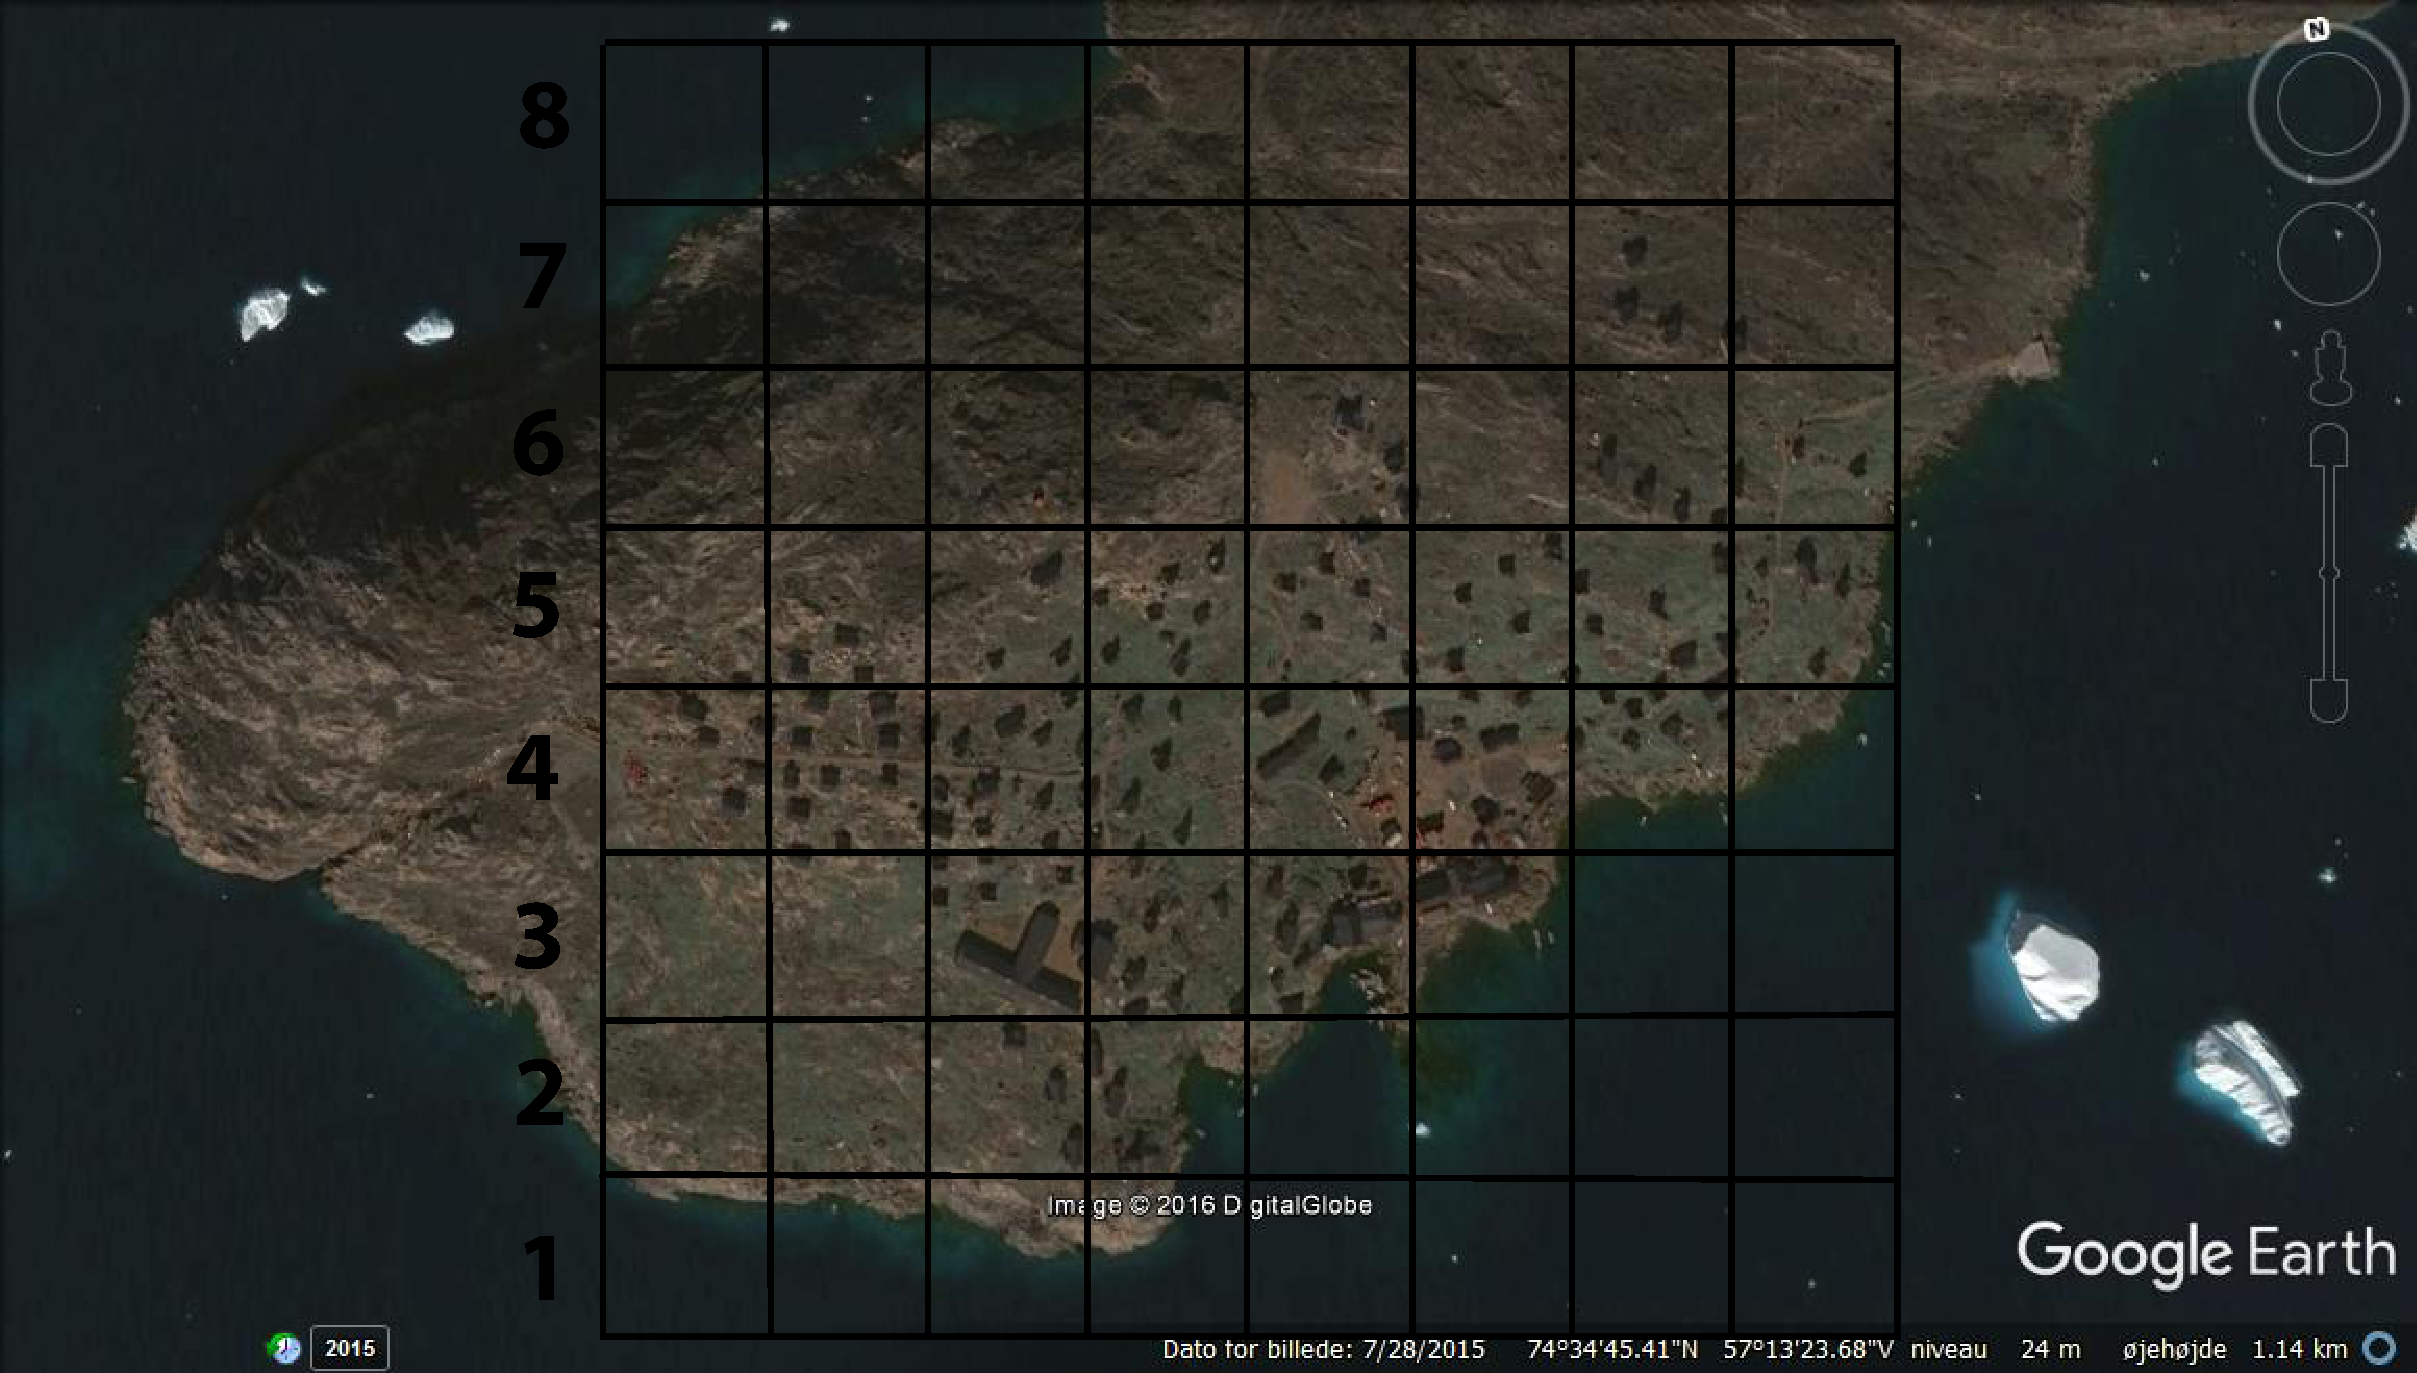
\includegraphics[width=0.8\textwidth]{figure/kullorsuaqGrid.pdf}
	\caption{Fordeling af Kullorsuaq. Hver tern har en opløsning på 100x100 m.}
	\label{fig:grid}
\end{figure} 

For at finde ud af, hvor meget af ressourcerne der skal tildeles til hver enkelt tern, skal antallet af brugere findes i hver tern. I tidligere afsnit \ref{sec:valgAfBygd} blev antallet af personer pr. hustand nævnt, som er 5,2 pr. husstand. Inden beregning af brugere i hver tern, antages at der er 3 brugere i hver hustand. Det eksakte antal huse i Kullorsuaq vides ikke, og optællingen sker ved at bruge Google Earth, hvor opløsningen ikke er bedst. Antallet af brugere hvor hver tern ses på tabel \ref{tab:antalPrTern}

\begin{table}[h]\label{tab:antalPrTern}
	\centering
    \begin{tabular}{|c|c|c|c|c|c|c|c|c|}
    \hline
    \textbf{y8} & 0  & 0  & 0  & 0  & 0  & 0  & 0  & 0  \\ \hline
    \textbf{y7} & 0  & 0  & 0  & 0  & 0  & 0  & \textbf{12} & 0  \\ \hline
    \textbf{y6} & 0  & 0  & 0  & 0  & \textbf{9}  & 0  & \textbf{12} & \textbf{9}  \\ \hline
    \textbf{y5} & 0  & \textbf{9}  & \textbf{9}  & \textbf{24} & \textbf{21} & \textbf{15} & \textbf{21} & \textbf{9}  \\ \hline
    \textbf{y4} & \textbf{18} & \textbf{30} & \textbf{33} & \textbf{21} & \textbf{21} & \textbf{15} & \textbf{21} & 0  \\ \hline
    \textbf{y3} & 0  & 0  & \textbf{12} & \textbf{24} & \textbf{12} & 0  & 0  & 0  \\ \hline
    \textbf{y2} & 0  & 0  & \textbf{9}  & \textbf{9}  & 0  & 0  & 0  & 0  \\ \hline
    \textbf{y1} & 0  & 0  & 0  & 0  & 0  & 0  & 0  & 0  \\ \hline
    -  & \textbf{x1} & \textbf{x2} & \textbf{x3} & \textbf{x4} & \textbf{x5} & \textbf{x6} & \textbf{x7} & \textbf{x8} \\ \hline
    \end{tabular}
    \caption{Antallet af brugere for hver tern.}
\end{table}

Antallet af alle brugere deles med den totale kapacitetsbehov for 2017, hvor at finde kapacitetsbehovet for hver tern. 
\begin{equation}
	kapBehovTern = \frac{antalBrugere}{kapBehovTotal}
\end{equation}
\begin{equation}
	KapBehovTern = \frac{375}{63,861 kbps}
	KapBehovTern = 5,87 kbps
\end{equation}

Kapacitetsbehovet for hver tern ganges for alle tern, og tallene kan ses på tabel \ref{tab:kapBehovTern}
\begin{table}[h]\label{tab:kapBehovTern}
	\centering
    \begin{tabular}{|c|c|c|c|c|c|c|c|c|}
    \hline
    \textbf{y8} & 0      & 0      & 0      & 0      & 0      & 0     & 0      & 0     \\ \hline
    \textbf{y7} & 0      & 0      & 0      & 0      & 0      & 0     & \textbf{70,44}  & 0     \\ \hline
    \textbf{y6} & 0      & 0      & 0      & 0      & \textbf{52,83}  & 0     & \textbf{70,44}  & \textbf{52,83} \\ \hline
    \textbf{y5} & 0      & \textbf{52,83}  & \textbf{52,83}  & \textbf{140,88} & \textbf{123,27} & \textbf{88,05} & \textbf{123,27} & \textbf{52,83} \\ \hline
    \textbf{y4} & \textbf{105,66} & \textbf{176,10} & \textbf{193,71} & \textbf{123,27} & \textbf{123,27} & \textbf{88,05} & \textbf{123,27} & 0     \\ \hline
    \textbf{y3} & 0      & 0      & \textbf{70,44}  & \textbf{140,88} & \textbf{70,44}  & 0     & 0      & 0     \\ \hline
    \textbf{y2} & 0      & 0      & \textbf{52,83}  & \textbf{52,83}  & 0      & 0     & 0      & 0     \\ \hline
    \textbf{y1} & 0      & 0      & 0      & 0      & 0      & 0     & 0      & 0     \\ \hline
    -  & \textbf{x1}     & \textbf{x2}     & \textbf{x3}     & \textbf{x4}     & \textbf{x5}     & \textbf{x6}    & \textbf{x7}     & \textbf{x8}    \\ \hline
    \end{tabular}
    \caption{Kapacitetsbehovet for hver tern i kbps.}
\end{table}